\documentclass[12pt]{article}

% Package for including images
\usepackage{graphicx}
% Package for database diagrams and other diagrams
\usepackage{tikz}
% Package for hyperlinks
\usepackage{hyperref}
% Package for figure placement
\usepackage{float}

\title{FarmClash - Software Product Technical Report}
\author{Camille De Vuyst, Joren Van der Sande, Thomas De Volder,\\ Faisal Ettarrahi, Ferhat Van Herck, Siebe Mees}
\date{\today}

\begin{document}

\maketitle
\tableofcontents
\newpage

\section{Introduction}
\subsection{Purpose}
This document serves as the comprehensive manual for FarmClash, a strategic resource management and town builder game that combines elements of classic farm management and competitive interactions among players. It details the game’s design, database schema, and functionality to assist developers, testers, and users in understanding and interacting with the system effectively.

\subsection{Scope}
This manual is intended to articulate the functionalities of FarmClash, providing guidance on the gameplay mechanics, user interaction, architecture, and technology stack utilized in the development. It covers various components including the player interface, game economy, resource management, defensive and offensive strategies, and the multiplayer aspects of the game. The intended audience for this document includes the development team, testers for quality assurance, and end-users who seek a deeper understanding of the game’s underlying mechanics.

\section{System Overview}
FarmClash is an ambitious and intricately designed game that challenges players to build and manage a farm in a competitive environment. The overarching design incorporates modern web technologies and follows a client-server architecture to deliver a real-time gaming experience.
\subsection{TODO: High-Level Architecture}
\begin{itemize}
    \item \textbf{Client}: Utilizes React, HTML, JavaScript, and CSS to create a dynamic and responsive user interface. The client side is responsible for presenting the game world, capturing user inputs, and providing interactive feedback.
    \item \textbf{Server}: Implements a RESTful API using Node.js and Express to handle game logic, data storage, and communication between clients. The server side processes user actions, updates the game state, and enforces the game rules.
    \item \textbf{Database}: Utilizes a relational database (e.g., MySQL) to store user data, game state, and other essential information. The database is accessed by the server to persist game progress and maintain data consistency.
    \item \textbf{Communication}: The client-server communication is facilitated through HTTP requests and responses, enabling real-time updates and synchronization of game state across multiple clients.
\end{itemize}

\subsection{TODO: Main Components}
\begin{itemize}
    \item \textbf{User Interface}: The user interface provides players with a visual representation of the game world, including farms, buildings, crops, and other elements. It allows users to interact with the game, manage resources, and make strategic decisions.
    \item \textbf{Game Mechanics}: The game logic governs the rules of the game, including resource management, building construction, crop growth, and player interactions. It enforces the game mechanics and ensures a fair and engaging gameplay experience.
    \item \textbf{Defensive and Offensive Strategies}: The database management system stores and retrieves game data, including user information, farm details, building configurations, and crop statistics. It maintains data integrity and supports complex queries to drive game mechanics.
    \item \textbf{Social Interaction}: Networking enables communication between clients and the server, allowing players to interact with each other, engage in trade, and compete in various challenges. It ensures real-time updates and synchronization of game state across all connected clients.
    \item \textbf{Game Economy}: The game economy manages resources, currencies, and transactions within the game world. It establishes pricing mechanisms, trade systems, and reward structures to incentivize player engagement and progression.
    \item \textbf{Progression and Expansion}: Multiplayer functionality enables players to form alliances, compete in challenges, and engage in player-versus-player interactions. It fosters a sense of community and competition among players, enhancing the overall gaming experience.
\end{itemize}

\section{Database Design}
\subsection{Database Schema}
The database schema is designed to support a farming simulation game, featuring users, farms, buildings, crops, and other elements essential for gameplay. The schema consists of several interconnected tables, each serving a specific purpose within the game's ecosystem. Key relationships between tables are established through foreign keys, ensuring data integrity and facilitating complex queries that drive game mechanics.

% Including an image (Your diagram)
\begin{figure}[H]
 \centering
 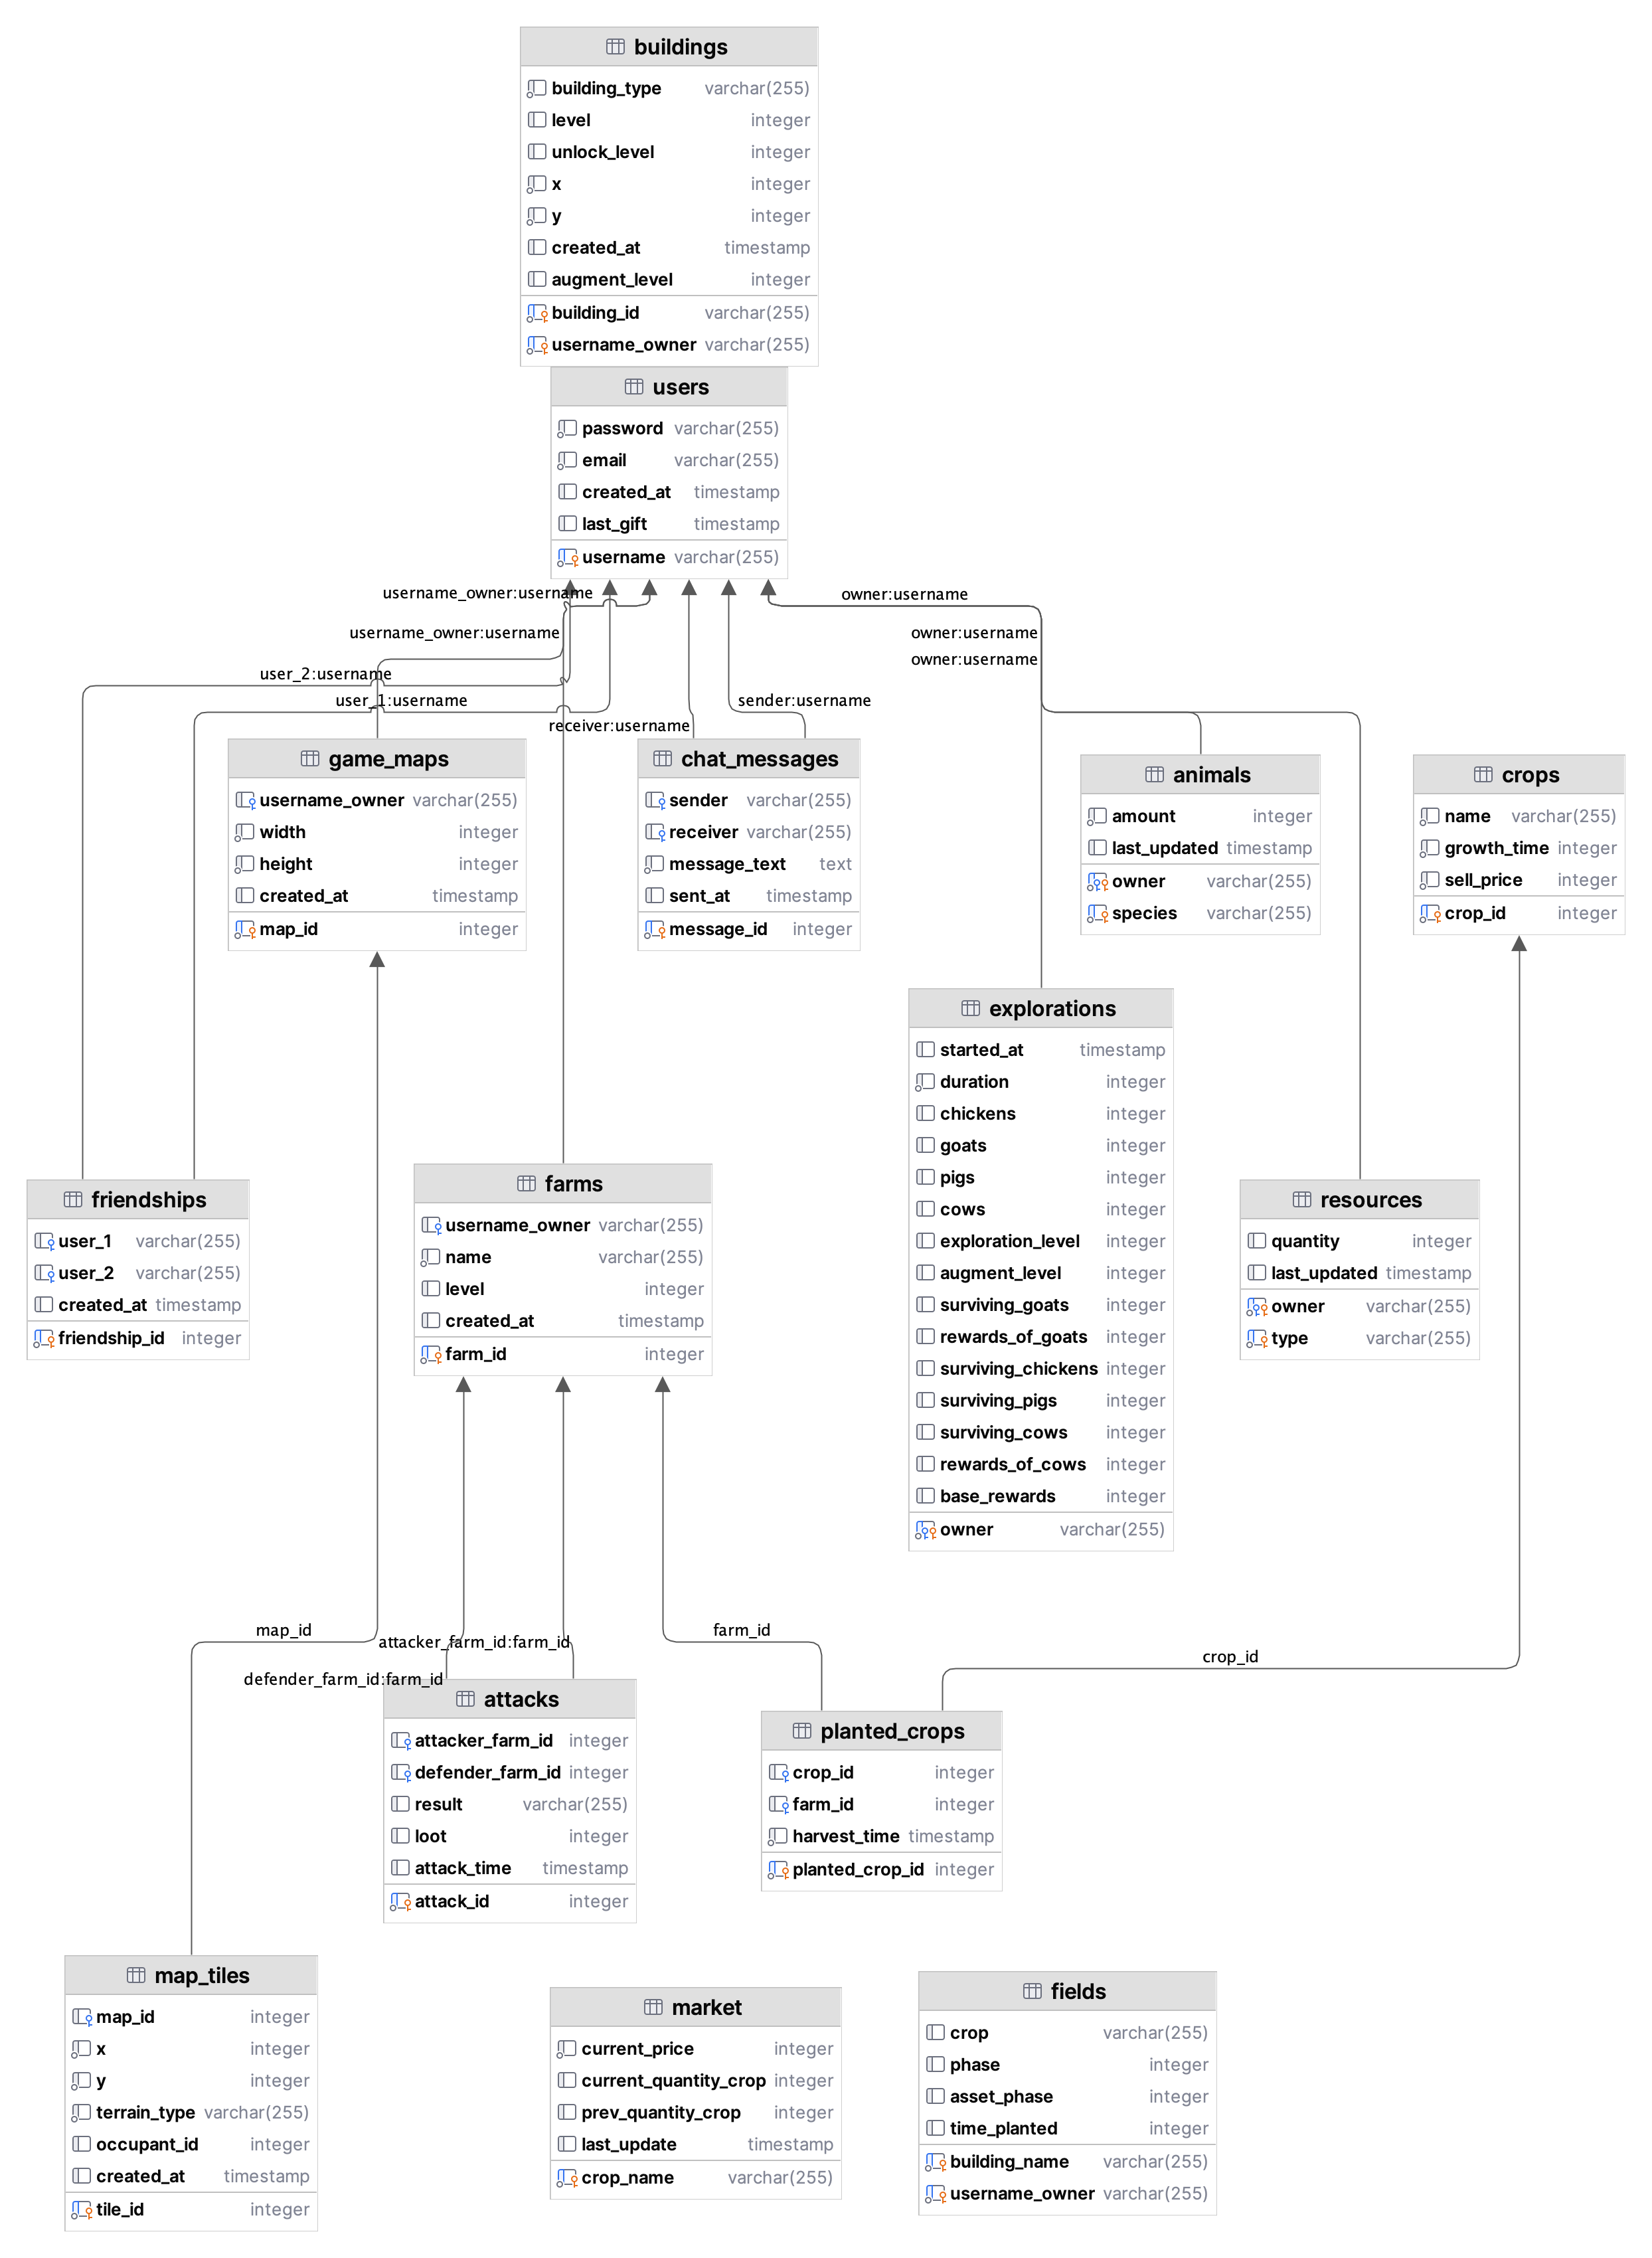
\includegraphics[width=0.8\textwidth]{img/db-diagram.png}
 \caption{Database schema diagram}
\end{figure}


\subsection{Table Descriptions}

\subsubsection{Users Table}
The users table stores information about players, including their username, password, email, and account creation date. Each user is uniquely identified by their username.

\subsubsection{Farms Table}
This table represents the farms owned by users. It includes a unique ID for each farm, the username of its owner (linked to the users table), the farm's name, its level, and the creation date.

\subsubsection{Buildings Table}
The buildings table tracks buildings on each farm, identified by a unique building ID. It stores the farm ID (linked to the farms table), the type of building, its level, and the creation date.

\subsubsection{Crops Table}
This table lists all available crop types in the game, including their name, growth time, and sell price. Each crop type is uniquely identified by a crop ID.

\subsubsection{Planted Crops Table}
The planted\textunderscore crops table keeps track of crops planted on farms, including a unique ID for each planted crop, the crop ID (linked to the crops table), the farm ID (linked to the farms table), and the harvest time.

\subsubsection{Market Table}
(Optional) The market table is designed for dynamic pricing of crops. It includes a market ID, crop ID (linked to the crops table), the current price of the crop, and the last update time.

\subsubsection{Resources Table}
This table tracks various resources owned by users, such as money or inventory items. It includes a resource ID, the owner's username (linked to the users table), the type of resource, and the quantity.

\subsubsection{Attacks Table}
(If implementing the attack feature) The attacks table records attacks between farms, including the attack ID, attacker and defender farm IDs (linked to the farms table), the result of the attack, the loot stolen, and the attack time.

\subsubsection{Friendships Table}
The friendships table tracks friendships between users, including a friendship ID, the usernames of the friends (linked to the users table), and the creation date of the friendship.

\subsubsection{Chat Messages Table}
This table stores chat messages sent between users, with a message ID, sender and receiver usernames (linked to the users table), the message text, and the time sent.

\subsubsection{Game Maps Table}
The game\textunderscore maps table stores information about game maps owned by users, including a map ID, the owner's username (linked to the users table), the map's width and height, and the creation date.

\subsubsection{Map Tiles Table}
This table tracks individual tiles within game maps, including a tile ID, the map ID (linked to the game\textunderscore maps table), the x and y coordinates of the tile, the terrain type, an optional occupant ID, and the creation date.

\section{Functionality Description}
\subsection{Login Feature}
Detail the implementation of the Login feature, including any relevant code snippets, algorithms, or flowcharts.
\subsubsection{Code Snippets}
\subsubsection{Flowchart}
\begin{figure}[H]
 \centering
 \includegraphics[width=0.8\textwidth]{img/login-flowchart.png}
 \caption{Login flowchart}
\end{figure}
% Example for including a code snippet
% \begin{verbatim}
%   Code snippet here
% \end{verbatim}

\subsection{Other Features}
Describe other features of the software, following the same format as the Login feature section. Include diagrams or flowcharts if applicable.

\section{Development and Implementation}
Discuss how the project was developed and implemented, emphasizing the involvement of each team member in various phases such as coding, testing, and documentation.

\section{Conclusion}
Summarize the key points of the manual and the software product's capabilities.

\end{document}
